% \documentclass[handout]{beamer}
% \usepackage{pgfpages}
% \pgfpagesuselayout{2 on 1}[a4paper,border shrink=5mm]
% \usecolortheme{lily}

\documentclass{beamer}
\usecolortheme{orchid}

\usepackage[utf8]{inputenc}
\usepackage[german]{babel}
\usepackage{hyperref}
\usepackage{tikz}
\usetikzlibrary{matrix}
\usepackage{tikz-uml}
\usepackage[edges]{forest}
\usepackage{cancel}
\PassOptionsToPackage{dvipsnames}{xcolor}
\usepackage{minted}


\newcommand{\btVFill}{\vskip0pt plus 1filll}
\newcommand*{\Scale}[2][4]{\scalebox{#1}{$#2$}}%
\newcommand*{\TakeFourierOrnament}[1]{{%
\fontencoding{U}\fontfamily{futs}\selectfont\char#1}}
\newcommand*{\danger}{\TakeFourierOrnament{66}}

\definecolor{CodeBackground}{HTML}{F5F5F0}
\usemintedstyle{manni}

\title[DFB Predict]{Fußball-Bundesliga Spielprognosen}
\subtitle{Vanessa Tsingunidis, Moritz Kniebel und Tim Fischer}
\date{07.02.2019}

\begin{document}
    \setlength{\abovedisplayskip}{0pt}
    \setlength{\belowdisplayskip}{0pt}
    \setlength{\abovedisplayshortskip}{0pt}
    \setlength{\belowdisplayshortskip}{0pt}
    \begin{frame}
        \titlepage
    \end{frame}
    \begin{frame}
        \frametitle{Agenda}
        4 diskrete Teilbereiche:
        \begin{enumerate}
            \item Repräsentation der Daten
            \item Beschaffung der Daten
            \item Vorhersage
            \item Interaktion
        \end{enumerate}
        \begin{itemize}
            \item Focus: Designentscheidungen
        \end{itemize}
    \end{frame}
    \begin{frame}
        \frametitle{Repräsentation der Daten}
        Ansprüche:
        \begin{itemize}
            \item mehr als nur \textit{bei Runtime}
            \item keine Duplikate
            \item einfach unterteilbar/abfragbar
            \item effizient
        \end{itemize}
        $\Rightarrow$ Relationale Datenbank\\\\
        Designvorgabe:
        \begin{itemize}
            \item unabhängig von Webframeworks
            \item möglichst wenig Overhead
            \item einfache Darstellung in Code
        \end{itemize}
        $\Rightarrow$ ORM via SQLAlchemy (\url{https://www.sqlalchemy.org/})
    \end{frame}
    \begin{frame}
        \frametitle{Repräsentation der Daten: DB-Model}
        \begin{center}
        \begin{tikzpicture}[scale=0.8, every node/.style={transform shape}]
            \umlclass[x=-5, y=5]{Match}{
                date : DateTime \\
                is\_finished : bool \\
                group : Group \\
                host\_points : int \\
                guest\_points : int \\
            }{
                host : Team \\
                guest : Team \\
            }
            \umlclass[x=5, y=5]{Team}{
                name : str \\
                seasons : List[Season] \\
            }{
                matches : List[Match] \\
            }
            \umlclass[x=0, y=5]{MatchParticipation}{
                team : Team \\
                match : Match \\
                hosted : bool \\
            }{

            }
            \umlclass[x=-5, y=0]{Group}{
                order\_id : int \\
                matches : List[Match] \\
            }{

            }
            \umlclass[x=5, y=0]{Season}{
                year : int \\
                groups : List[Group] \\
                teams : List[Team] \\
            }{

            }

            \umlcompo{Season}{Team}
            \umlcompo{Season}{Group}
            \umlcompo{Group}{Match}
            \umlcompo[mult1=1, mult2=2]{Match}{MatchParticipation}
            \umlcompo[mult1=0..*, mult2=1]{MatchParticipation}{Team}
        \end{tikzpicture}
        \end{center}
    \end{frame}
    \begin{frame}[fragile]
        \frametitle{Repräsentation der Daten: Datenselektion}
        \begin{alertblock}{Problem}
            Das Bauen/Bilden von Queries zur Auswahl von Spielen auf Basis deren Spieltag oder gar von Teams auf Basis der Spielen, ist langwierig und kompliziert...
            \begin{minted}[fontsize=\tiny, autogobble, bgcolor=CodeBackground]{python3}
                Query(Team).join(
                    Team.seasons,
                    Team.match_participations,
                    MatchParticipation.match,
                    Match.group
                ).filter(
                    Match.is_finished,
                    ...
                )
            \end{minted}
        \end{alertblock}
    \end{frame}
    \begin{frame}[fragile]
        \frametitle{Repräsentation der Daten: Datenselektion \tiny{(\texttt{src/db/selectors.py})}}
        \begin{block}{Idee}
            Stellen wir eine derartige Auswahl als Zeitraum dar, welcher dann intern die Logik für das Erstellen der Queries enthält.
        \end{block}
        \begin{exampleblock}{Implementation}
            \begin{minted}[fontsize=\tiny, autogobble, bgcolor=CodeBackground]{python3}
                range_selector = RangeSelector(
                    start=RangePoint(year=2016, group=1),
                    end=RangePoint(year=2016, group=34)
                )

                with DB.get_session() as session:
                    print(*range_selector.build_team_query().with_session(session), sep="\n")
            \end{minted}
        \end{exampleblock}
    \end{frame}
    \begin{frame}
        \frametitle{Beschaffung der Daten}
        3 Möglichkeiten:
        \begin{enumerate}
            \item statischer Datensatz
            \item Web Scraping
            \item öffentliche API
        \end{enumerate}
        $\Rightarrow$ alle haben Vor- und Nachteile...
    \end{frame}
    \begin{frame}
        \frametitle{Beschaffung der Daten: statischer Datensatz}
        \begin{exampleblock}{Pro}
            \begin{itemize}
                \item kein Internetzwang
                \item kein zusätzlich Aufwand für die Datenaufbereitung
            \end{itemize}
        \end{exampleblock}
        \begin{alertblock}{Kontra}
            \begin{itemize}
                \item möglicher organisatorischer Aufwand
                \item erschwertes Verbreiten neuer Datensätze an Endnutzer
            \end{itemize}
        \end{alertblock}
    \end{frame}
    \begin{frame}
        \frametitle{Beschaffung der Daten: Web Scraping}
        \begin{exampleblock}{Pro}
            \begin{itemize}
                \item wenig organisatorischer Aufwand
                \item immer aktuelle Daten
            \end{itemize}
        \end{exampleblock}
        \begin{alertblock}{Kontra}
            \begin{itemize}
                \item eigene Parse-Arbeit
                \item zusätzlich Aufwand für die Datenaufbereitung
                \item Willkür der Anbieter
                \item Internetzwang
                \item Legalität
            \end{itemize}
        \end{alertblock}
    \end{frame}
    \begin{frame}
        \frametitle{Beschaffung der Daten: öffentliche API}
        \begin{exampleblock}{Pro}
            \begin{itemize}
                \item wenig organisatorischer Aufwand
                \item immer aktuelle Daten
                \item keine eigene Parse-Arbeit
            \end{itemize}
        \end{exampleblock}
        \begin{alertblock}{Kontra}
            \begin{itemize}
                \item \textit{zusätzlich Aufwand für die Datenaufbereitung}
                \item Willkür der Anbieter
                \item Internetzwang
            \end{itemize}
        \end{alertblock}
    \end{frame}
    \begin{frame}
        \frametitle{Beschaffung der Daten}
        3 Möglichkeiten:
        \begin{enumerate}
            \item {\color{gray}statischer Datensatz}
            \item {\color{gray}Web Scraping}
            \item öffentliche API (\url{https://www.openligadb.de})
        \end{enumerate}
    \end{frame}
    \begin{frame}
        \frametitle{Beschaffung der Daten: Dataprocessing-Pipeline}
        \begin{alertblock}{Problem}
            Wie bekommen wir die Daten aus der API-Response in die Datenbank?
        \end{alertblock}
    \end{frame}
    \begin{frame}[fragile]
        \frametitle{Beschaffung der Daten: Dataprocessing-Pipeline \tiny{(\texttt{src/acquisition/*})}}
        \begin{block}{Idee}
            Beschreiben wir für jedes Feld in den DB-Modellen, durch eine \textit{Konkatenation} von \textit{Transformationen}, wie man von dem Response aus zu dem jeweiligen Wert kommt.
        \end{block}
        \begin{exampleblock}{Implementation}
            \begin{minted}[fontsize=\tiny, autogobble, bgcolor=CodeBackground]{python3}
                pipeline: Pipeline[Model] = Pipeline({
                    MatchParticipation: {
                        "team": Get("Team") | GetOrCreate(Team, match_targets=["id"]),
                        "match_id": Get("MatchID"),
                        "hosted": Get("hosted"),
                    },
                    Team: {
                        "id": Get("TeamId"),
                        "name": If(
                            cond=lambda data: "ShortName" in data and data["ShortName"],
                            then=Get("ShortName"),
                            else_=Get("TeamName"),
                        )
                    },
                    ...
                })
            \end{minted}
        \end{exampleblock}
    \end{frame}
    \begin{frame}
        \frametitle{Vorhersage}
        \begin{enumerate}
            \item Poisson-Regression
            \item Dixon-Coles \tiny{(\url{http://web.math.ku.dk/~rolf/teaching/thesis/DixonColes.pdf})}
        \end{enumerate}
    \end{frame}
    \begin{frame}
        \frametitle{Poisson-Regression: Basis}
        \begin{block}{Kernidee}
            Die Anzahl der geschossene Tore eines Teams in einem Spiel kann mittels der Angriffs- und Verteidigungsstärken der beiden Teams ermittelt werden.
        \end{block}
        \begin{block}{Annahme}
            \begin{align*}
                X_{i,j} &\approx Poisson(\alpha_i\beta_j\gamma)\\
                Y_{i,j} &\approx Poisson(\alpha_j\beta_i)
            \end{align*}
            \begin{itemize}
                \item $\alpha_t$ und $\beta_t$ stellen jeweils die Angriffs- und Verteidigungsstärke des Team $t$ dar
                \item $i$ und $j$ stellen die beiden Teams dar
                \item $\gamma$ stellt den durchschnittlichen Heimvorteil dar
            \end{itemize}
        \end{block}
    \end{frame}
    \begin{frame}
        \frametitle{Poisson-Regression: Modell}
        \begin{block}{Bivariates Poisson}
            \begin{itemize}
                \item Anzahl der Tore der Heim- bzw. Gastmannschaft
            \end{itemize}
            \[
                P(X_{i,j} = x, Y_{i,j} = y) =
                \frac{e^{-\lambda}\lambda^{x}}{x!}\frac{e^{-\mu}\mu^{y}}{y!}
            \]\[
                \text{where }
                \lambda = \alpha_{i}\beta_{j}\gamma \hspace{.5cm}
                \mu = \alpha_{j}\beta_{i}
            \]
        \end{block}
    \end{frame}
    \begin{frame}
        \frametitle{Poisson-Regression: Modell}
        \begin{block}{Likelyhood Funktion}
            \[
                L(\alpha_i, \beta_i, \gamma; i = 0,\hdots, |T|) =
                \prod_{m = 0}^{|M|} \frac{e^{-\lambda}\lambda^{x_m}}{x_m!}\frac{e^{-\mu}\mu^{y_m}}{y_m!}
            \]\[
                \text{where }
                \lambda_m = \alpha_{i_m}\beta_{j_m}\gamma \hspace{.5cm}
                \mu_m = \alpha_{j_m}\beta_{i_m}
            \]
            \begin{itemize}
                \item $i_m$ und $j_m$ stellen die Teams im Spiel $m$ dar
                \item $x_m$ und $y_m$ stellen die geschossenen Tore im Spiel $m$ dar
            \end{itemize}
        \end{block}
    \end{frame}
    \begin{frame}
        \frametitle{Dixon-Coles: Basis}
        \begin{block}{Annahme}
            \begin{itemize}
                \item Poisson überschätzt in den niedrigen Torbereichen
                \item Nicht alle Daten sind gleich viel Wert, je jünger sie sind desto relevanter sind sie.
            \end{itemize}
        \end{block}
    \end{frame}
    \begin{frame}
        \frametitle{Dixon-Coles: Modell}
        \begin{block}{$\tau$-Funktion}
            \begin{itemize}
                \item Diese Funktion stellt den Grad dar, um welchen die Wahrscheinlichkeiten für niedrige Torergebnisse ($<2$) angepasst werden.
            \end{itemize}
            \[
                \tau_{\lambda,\mu}(x, y) =
                \begin{cases}
                    1 - \lambda\mu\rho, &\text{if } x = y = 0\\
                    1 + \lambda\rho, &\text{if } x = 0, y = 1\\
                    1 + \mu\rho, &\text{if } x = 1, y = 0\\
                    1 - \rho, &\text{if } x = 1, y = 1\\
                    1, &\text{otherwise}
                \end{cases}
            \]\vspace{.3cm}\[
                D(X_{i,j} = x, Y_{i,j} = y) =
                \tau_{\lambda,\mu}(x, y)
                \frac{e^{-\lambda}\lambda^{x}}{x!} \frac{e^{-\mu}\mu^{y}}{y!}
            \]
            \begin{itemize}
                \item $\rho$ stellt hier eine Korrekturfaktor dar
            \end{itemize}
        \end{block}
    \end{frame}
    \begin{frame}
        \frametitle{Dixon-Coles: Modell}
        \begin{block}{Likleyhood with Time Decay}
            \begin{itemize}
                \item Nicht alle Daten haben die gleiche Relevanz.
            \end{itemize}
            \[
                \phi(t) = e^{\xi t}
            \]\vspace{1pt}\[\Scale[.8]{
                L(\alpha_i, \beta_i, \rho, \gamma; i = 0,\hdots, |T|) =
                \prod_{m = 0}^{|M|} \left\{
                    \tau_{\lambda_m,\mu_m}(x_m, y_m) \dfrac{e^{-\lambda_m}\lambda_m^{x_m}}{x_m!} \dfrac{e^{-\mu_m}\mu_m^{y_m}}{y_m!}
                \right\}^{\phi(t_0 - t_m)}
            }\]\vspace{1pt}\[
                \text{where }
                \lambda_m = \alpha_{i_m}\beta_{j_m}\gamma \hspace{.5cm}
                \mu_m = \alpha_{j_m}\beta_{i_m}
            \]
            \begin{itemize}
                \item $t_0$ stellt den Zeitpunkt des jüngsten Spiels dar
                \item $t_m$ stellt den Zeitpunkt des Spiels $m$ dar
                \item $\xi$ stellt einen Faktor zur Kontrolle des Relevanzabfalls dar ($\xi = 0.0065$)
            \end{itemize}
        \end{block}
    \end{frame}
    \begin{frame}
        \frametitle{Dixon-Coles: Modell}
        \begin{block}{Maximierung der Likelyhood Funktion}
            Initialwerte:
            \begin{itemize}
                \item Angriff: $0.01 \rightarrow \alpha$
                \item Verteidigung: $-0.08 \rightarrow \beta$
                \item Korrektur: $0.03 \rightarrow \rho$
                \item Heimvorteil: $0.06 \rightarrow \gamma$
            \end{itemize}
            Einschränkungen:
            \begin{itemize}
                \item $\frac{1}{|T|} \sum_i \alpha_i = 1$
            \end{itemize}
        \end{block}
    \end{frame}
    \begin{frame}
        \frametitle{Vorhersage: Interpretation der Resultate}
        ...
    \end{frame}
    \begin{frame}
        \frametitle{Interaktion}
        3 Möglichkeiten:
        \begin{enumerate}
            \item CLI
            \item Web GUI
            \item Native GUI
        \end{enumerate}
    \end{frame}
    \begin{frame}
        \frametitle{Interaktion: GUI Optionen}
        \begin{columns}
            \column{0.5\textwidth}
            Web Interface
            \begin{exampleblock}{Pro}
                \begin{itemize}
                    \item flexible
                    \item \textit{''hostbar''}
                \end{itemize}
            \end{exampleblock}
            \begin{alertblock}{Kontra}
                \begin{itemize}
                    \item extra Libraries
                    \item HTML/CSS (JS)
                \end{itemize}
            \end{alertblock}
            
            \column{0.5\textwidth}
            Native Interface
            \begin{exampleblock}{Pro}
                \begin{itemize}
                    \item in Python-\textit{''STL''}
                    \item einfacher Systemzugriff
                \end{itemize}
            \end{exampleblock}
            \begin{alertblock}{Kontra}
                \begin{itemize}
                    \item Komplexere Code
                    \item nicht so hübsch
                \end{itemize}				
            \end{alertblock}	
        \end{columns}
    \end{frame}
    \begin{frame}
        \frametitle{Interaktion}
        3 Möglichkeiten:
        \begin{enumerate}
            \item CLI
            \item {\color{gray}Web GUI}
            \item Native GUI
        \end{enumerate}
        $\Rightarrow$ Click \small{(\url{https://palletsprojects.com/p/click/})}\\
        $\Rightarrow$ tkinter \small{(\url{https://docs.python.org/3.5/library/tkinter.html})}
    \end{frame}
    \begin{frame}
        \frametitle{Interaktion: CLI \tiny{(\texttt{src/cli.py})}}
        \begin{block}{Layout}
            \begin{forest}
            for tree={
                font=\footnotesize\ttfamily,
                text=white,
                if level=0
                    {fill=darkgray}
                    {fill=gray},
                rounded corners=4pt,
                grow'=0,
                child anchor=west,
                parent anchor=south,
                anchor=west,
                calign=first,
                edge={lightgray,rounded corners,line width=1pt},
                edge path={
                    \noexpand\path [draw, \forestoption{edge}]
                    (!u.south west) +(6pt,0) |- (.child anchor)\forestoption{edge label};
                },
                before typesetting nodes={
                if n=1
                    {insert before={[,phantom]}}
                    {}
                },
                fit=band,
                s sep=5pt,
                before computing xy={l=15pt},
            }
            [cli \tiny{\textit{DFB Predict}}
                [currentmatches \tiny{\textit{retrieve list of matches in current group}}]
                [db \tiny{\textit{management of the local database}}
                    [download \tiny{\textit{download seasons}}]
                    [drop \tiny{\textit{drop all data}}]
                    [query \tiny{\textit{check data}}
                        [seasons]
                        [teams]
                        [matches]
                    ]
                ]
                [predict \tiny{\textit{predict single match}}]
                [ui \tiny{\textit{launch gui}}]
            ]
            \end{forest}
        \end{block}
    \end{frame}
    \begin{frame}
        \frametitle{Interaktion: Data Tab}
        \begin{block}{Funktion}
            \begin{itemize}
                \item Herrunterladen neuer Daten
                \item Bauen neuer Modelle
                \item Laden/Speichern existierender Modelle
            \end{itemize}
        \end{block}
        \center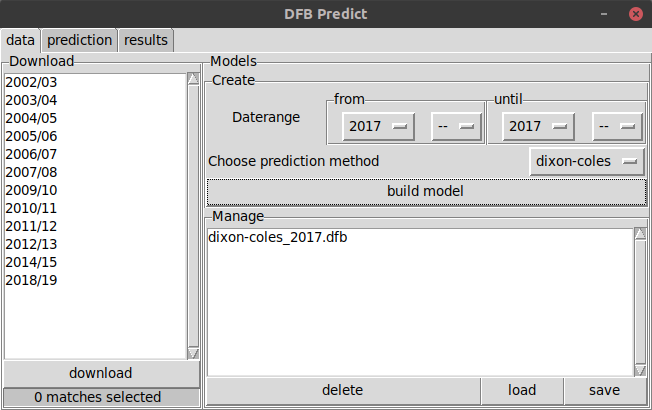
\includegraphics[scale=.3]{gui_imgs/001.png}
    \end{frame}
    \begin{frame}
        \frametitle{Interaktion: Prediction Tab}
        \begin{block}{Funktion}
            \begin{itemize}
                \item Spezifische Spiele vorhersagen
                \item Aktuellen Spieltag vorhersagen
                \item Spieltag aus der Datenbank vorhersagen
            \end{itemize}
        \end{block}
        \center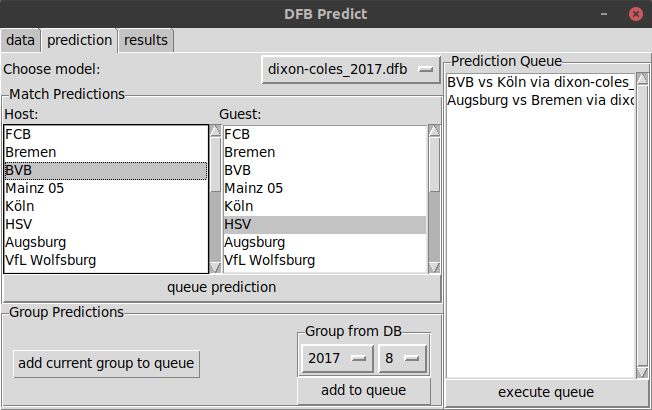
\includegraphics[scale=.3]{gui_imgs/002.png}
    \end{frame}
    \begin{frame}
        \frametitle{Interaktion: Result Tab}
        \begin{block}{Funktion}
            \begin{itemize}
                \item Vorhersagen begutachten
            \end{itemize}
        \end{block}
        \center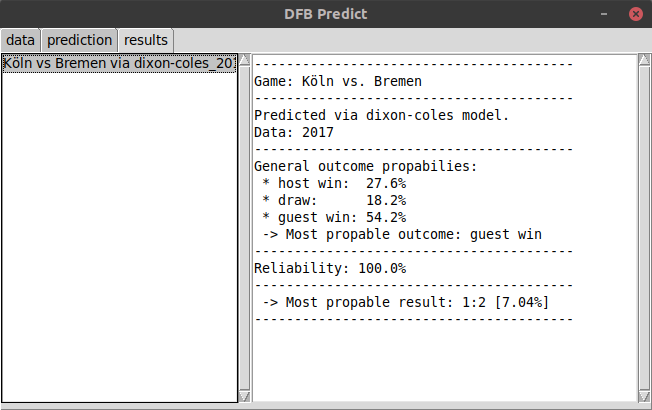
\includegraphics[scale=.3]{gui_imgs/003.png}
    \end{frame}
\end{document}